\documentclass[a4paper]{article}

\usepackage[T2A]{fontenc}
\usepackage[utf8]{inputenc}
\usepackage[russian]{babel}


\usepackage{graphicx}
\usepackage{float}
\usepackage{mathtools}
\usepackage{wrapfig}
\usepackage{amsfonts, amssymb, amsmath, latexsym}
\usepackage{nicefrac}
\usepackage{hhline}
\usepackage{multirow}
\usepackage[colorinlistoftodos,bordercolor=orange,backgroundcolor=orange!20,linecolor=orange,textsize=scriptsize]{todonotes}
\usepackage[colorlinks=true,linkcolor=blue,citecolor=blue]{hyperref}       % hyperlinks
\usepackage{nicefrac}       % compact symbols for 1/2, etc.
\usepackage{nameref}
\usepackage{booktabs}       % professional-quality tables

\usepackage{algorithm}
\usepackage{algpseudocode}

\usepackage{xcolor, colortbl}
\usepackage{etoolbox}

% \graphicspath{ {./} }

\usepackage[verbose=true,letterpaper]{geometry}

\newgeometry{
    textheight=9in,
    textwidth=5.5in,
    top=1in,
    headheight=12pt,
    headsep=25pt,
    footskip=30pt
}

\usepackage{epigraph}

%

\newcommand{\argmin}{\mathop{\arg\!\min}}
\newcommand{\argmax}{\mathop{\arg\!\max}}

\newcommand{\Var}{\mathbb{V}}
\newcommand{\Exp}{\mathbb{E}}
\newcommand{\Cov}{\text{Cov}}
\newcommand{\makebold}[1]{\boldsymbol{#1}}
\newcommand{\mean}[1]{\overline{#1}}
\newcommand{\eps}{\varepsilon}
\renewcommand{\epsilon}{\varepsilon}

\newcommand{\partfrac}[2]{\frac{\partial #1}{\partial #2}}
\newcommand{\ttt}[1]{\texttt{#1}}
\newcommand{\term}[1]{\textbf{#1}}

\newcommand{\la}{\langle}
\newcommand{\ra}{\rangle}

\newcommand{\lp}{\left(}
\newcommand{\rp}{\right)}
\newcommand{\lf}{\left\{}
\newcommand{\rf}{\right\}}
\newcommand{\ls}{\left[}
\newcommand{\rs}{\right]}
\newcommand{\lv}{\left|}
\newcommand{\rv}{\right|}

\newcommand*{\affaddr}[1]{#1} % No op here. Customize it for different styles.
\newcommand*{\affmark}[1][*]{\textsuperscript{#1}}


\usepackage{amsthm}

\theoremstyle{definition}
\newtheorem{definition}{Определение}[section]

\newtheorem{exercise}{Задача}[section]

\newtheorem*{solution}{Решение}
\theoremstyle{remark}
\newtheorem*{remark}{Remark}

\makeatletter
\renewcommand{\l@section}{\@dottedtocline{1}{0em}{2.1em}}
\makeatother

% \setlength\epigraphwidth{.8\textwidth}
\setlength\epigraphrule{0pt}

\title{Работа 3.1.3 \\ Измерение магнитного поля Земли}
\author{Шарапов Денис, Б05-005}
\date{}

\usepackage{fancyhdr}
\pagestyle{fancy}
\fancyhf{}
\rhead{Работа 3.1.3}
\lhead{}
\cfoot{\thepage}
\usepackage{subcaption}
\usepackage[font={small}]{caption}

\begin{document}

    \maketitle
    \tableofcontents
    \newpage
    
\section{Аннотация}

 \textbf{Цель работы:} определить характеристики шарообразных неодимовых магнитов и, используя законы взаимодействия магнитных моментов с полем, измерить горизонтальную и вертикальную составляющие индукции магнитного поля Земли и магнитное наклонение. \\
 
 \noindent \textbf{В работе используются:} : 12 одинаковых неодимовых магнитных шариков, тонкая нить для изготовления крутильного маятника, медная проволока диаметром $(0,5 – 0,6)$ мм, электронные весы, секундомер, измеритель магнитной индукции АТЕ-8702, штангенциркуль, брусок из немагнитного материала $(25 \times 30 \times 60$ $\text{мм}^3$), деревянная линейка, штатив из немагнитного материала; дополнительные неодимовые магнитные шарики $(\sim 20 \text{шт}.)$ и неодимовые магниты в форме параллелепипедов (2 шт.), набор гирь и разновесов
 
 \section{Теоретические сведения}
 
 \subsection{Точечный магнитный диполь}
 
 Простейший магнитный диполь может быть образован витком с током или постоянным магнитом. По определению, магнитный момент $\vec{P_m}$ тонкого витка площадью $S$ с током $I$ равен: $$\vec{P_m} = \frac{I}{c}\vec{S} = \frac{I}{c}S \vec{n},$$
 где $c$ --- скорость света в вакууме, $\vec{S} = S\vec{n}$ --- вектор площади контура, образующий  направлением тока правовинтовую систему, $\vec{n}$ --- единичный вектор нормали к площадке $S$ (это же направление $\vec{P_m}$ принимается за направление $S \rightarrow N$ от южного к северному полюсу).
 
 Магнитное поле точечного диполя определяется по формуле, аналогичной формуле для поля элементарного электрического диполя: $$\vec{B} = 3\frac{(\vec{P_m}, \vec{r})\vec{r}}{r^5} - \frac{\vec{P_m}}{r^3}.$$
 
 В магнитном поле с индукцией $\vec{B}$ на точечный магнитный диполь $\vec{P_m}$ действует механический момент сил: $$\vec{M} = \vec{P_m} \times \vec{B}.$$
 
 Магнитный диполь в магнитном поле обладает энергией: $$W = -(\vec{P_m}, \vec{B}).$$
 
 Зная магнитные моменты $P_1$ и $P_2$ двух небольших постоянных магнитов, можно рассчитать силу их взаимодействия. Если магнитные моменты $P_1 = P_2 = P_m$ двух одинаковых небольших магнитов направлены вдоль соединяющей их прямой, а расстояние между ними равно $r$, то магниты взаимодействуют с силой: $$F = P_m \frac{\partial B}{\partial r} = P_m \frac{\partial (2P_m / r^3)}{\partial r} = -6\frac{P_{m}^{2}}{r^4}.$$
 
\subsection{Неодимовые магнитные шары}

Магнитное поле однородно намагниченного шара радиуса $R$ на расстояниях $r \geq R$ от центра шара совпадает с полем точечного магнитного диполя $\vec{P_m}$, равного полному магнитному моменту шара и расположенного в его центре.

По определению намагниченность --- это магнитный момент единицы объёма. Для однородно намагниченного шара намагниченность, очевидно, равна: $$\vec{p_m} = \frac{\vec{P_m}}{V},$$ где $V$ --- объем шара.

Индукция магнитного поля $\vec{B_p}$ на полюсах однородно намагниченного шара связана с величиной намагниченности $\vec{p_m}$ и с остаточной магнитной индукцией $\vec{B_r}$, формулой: $$\vec{B_p} = (8\pi/3)\vec{p_m} = (2/3)\vec{B_r}.$$


\subsection{Экспериментальное определение величины магнитного момента магнитных шариков}


\begin{wrapfigure}{r}{120pt}
    \centering
    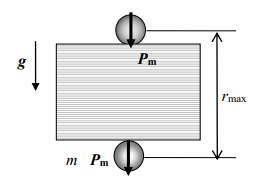
\includegraphics[width = 120pt]{image/pic1.png}
\end{wrapfigure}

При максимальном расстоянии сила тяжести шариков равна силе их магнитного притяжения: $$\frac{6P_m^2}{r_{max}^4} = mg, \quad P_m = \sqrt{ \frac{mgr^4_{max}}{6} }.$$ 

Максимальная величина индукции наблюдается на полюсах: $$\vec{B_p} = \frac{2\vec{P_m}}{R^3}.$$

\subsection{Измерение горизонтальной составляющей индукции магнитного поля Земля}

\begin{wrapfigure}{r}{120pt}
    \centering
    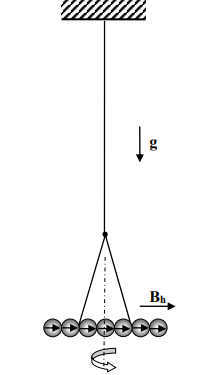
\includegraphics[width = 120pt]{image/pic2.png}
\end{wrapfigure}

Магнитное поле Земли в настоящей работе определяется по периоду крутильных колебаний магнитной стрелки вокруг вертикальной оси.

Период крутильных колебаний $$T = 2\pi\sqrt{ \frac{I_n}{P_0B_h} } = 2\pi\sqrt{ \frac{I_n}{nP_mB_h} },$$ где $P_0 = nP_m$ --- полный магнитный момент магнитной стрелки, составленной из $n$ шариков. 

Момент инерции стрелки, состоящей из $n$ шариков: $$I_n = \frac{1}{12}n^3md^2.$$ 

В приближении период колебаний маятника оказывается пропорциональным числу шаров $n$, составляющих стрелку: $$T(n) = \pi n\sqrt{ \frac{md^2}{3P_mB_h} }.$$

\subsection{Измерение вертикальной составляющей индукции магнитного поля Земли}

\begin{wrapfigure}{r}{180pt}
    \centering
    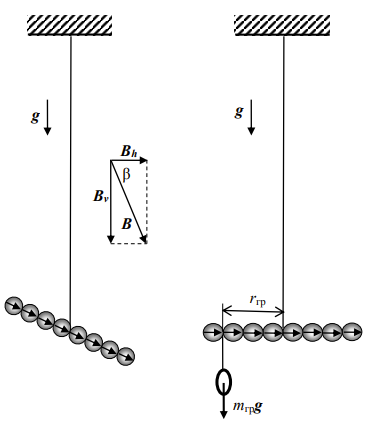
\includegraphics[width = 140pt]{image/pic3.png}
\end{wrapfigure}

С помощью небольшого дополнительного грузика стрелку можно выровнять, расположив её горизонтально: в этом случае момент силы тяжести груза относительно точки подвеса будет равен моменту сил, действующих на стрелку со стороны магнитного поля Земли. Если масса уравновешивающего груза равна $m_{\text{гр}}$, плечо силы тяжести $r_{\text{гр}}$, а полный магнитный момент стрелки $P_0 = nP_m$, то в равновесии: $$m_{\text{гр}}gr_{{\text{гр}}} = P_0B_v = nP_mB_v,$$ где $B_v$ --- вертикальная составляющая поля Земли. Видно, что момент $M(n)$ силы тяжести уравновешивающего груза пропорционален числу $n$ шариков, образующих магнитную стрелку: $$M(n) = An,$$ где $A = P_mB_v$.

\section{Результаты измерений и обработка данных}

\subsection{Определение магнитного момента}

Взвесим шарики на весах и определим их диаметр. Затем выясним, на каком максимальном расстоянии $r_{max}$ шарики удерживают друг друга в поле тяжести Земли. Результаты измерений занесём в таблицу 1.

\begin{table}[h!]
    \centering
    \begin{tabular}{|c|c|c|}
    \hline
    $m$, г            & $d$, мм          & $r_{max}$, мм      \\ \hline
    $0.850 \pm 0,001$ & $6,10 \pm 0,01$ & $19,00 \pm 0,01$ \\ \hline
    \end{tabular}
    \caption{Геометрические размеры шариков}
    \end{table}


Рассчитаем величину магнитного момента магнитика $P_m$, величину намагниченности материала шариков $p_m$, величину магнитного поля $B_p$ на полюсах шарика, величину остаточной магнитной индукции $B_r$: 

\begin{table}[h!]
    \centering
    \begin{tabular}{|c|c|c|c|}
    \hline
    $P_m$, эрг/Гс       & $p_m$, Гс      & $B_p$, кГс       & $B_r$, кГс      \\ \hline
    $42,600 \pm  0,001$ & $358,4 \pm 10$ & $3,00 \pm 0,09 $ & $4,50 \pm 0,14$ \\ \hline
    \end{tabular}
    \end{table}

Измерим величину поля $B_p$ на полюсах шарика датчиком: $$B_p = 2,87 \pm 0,01 \;\text{кГс}.$$

\subsection{Определение горизонтальной составляющей}

Соберём крутильный маятник и исследуем зависимость периода $T$ крутильных колебаний стрелки от количества магнитных шариков $n$, составляющих стрелку. Измерения представлены в таблице 2.

\begin{table}[h!]
    \centering
    \begin{tabular}{|c|c|c|c|c|c|c|c|c|c|c|}
    \hline
    $n$, шт & 12  & 11  & 10  & 9   & 8   & 7   & 6   & 5   & 4   & 3   \\ \hline
    $T$, с  & 3,1 & 2,8 & 2,6 & 2,4 & 2,2 & 1,9 & 1,7 & 1,4 & 1,1 & 0,8 \\ \hline
    \end{tabular}
    \caption{Зависимость периода колебаний от количества шариков}
    \end{table}


    \begin{figure}[t]
        \centering
        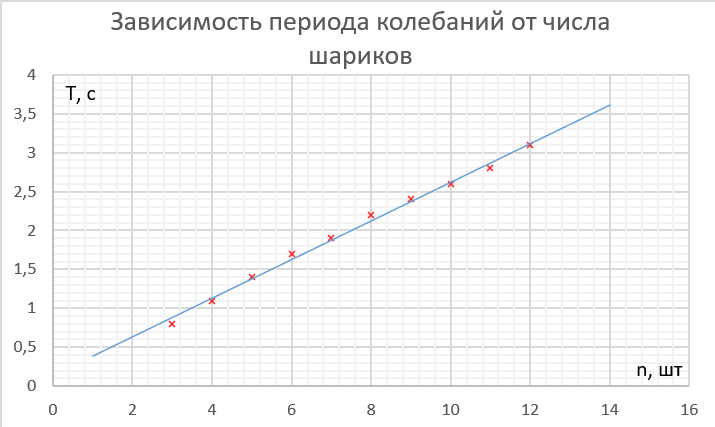
\includegraphics[width = 280pt]{image/graph1.png}
    \end{figure}


    Из МНК определяем коэффициент наклона $k$: $$k = 0,249 \pm 0,006 \; \text{с}.$$ По значению углового коэффициента рассчитаем величину горизонтальной составляющей $B_h$ магнитного поля Земли: $$B_h = 0,396 \pm  0,024\;\text{Гс}.$$


\subsection{Определение вертикальной составляющей}

Определим механический момент сил, деqствующих со стороны магнитного поля Земли на горизонтально расположенную магнитную стрелку. Для этого с помощью проволки уравновесим стрелку. С помощью весов определим массу уравновешивающего груза~$m_{\text{гр}}$. Результаты измерений приведены в таблице 3.

\begin{table}[h!]
    \centering
    \begin{tabular}{|c|c|c|}
    \hline
    $n$, шт & $m_{\text{гр}}$, г & $M$, дин$\cdot$см    \\ \hline
    10      & $0,195 \pm 0,001$                  & $573, 300 \pm 0,003$ \\ \hline
    8       & $0,206 \pm 0,001$                  & $484,500 \pm 0,004$  \\ \hline
    6       & $0,231 \pm 0,001$                  & $407,400 \pm 0,005$  \\ \hline
    4       & $0,313 \pm 0,001$                  & $368,100 \pm 0,005$  \\ \hline
    \end{tabular}
    \caption{Результаты измерения механического момента}
    \end{table}

    \begin{figure}[h!]
        \centering
        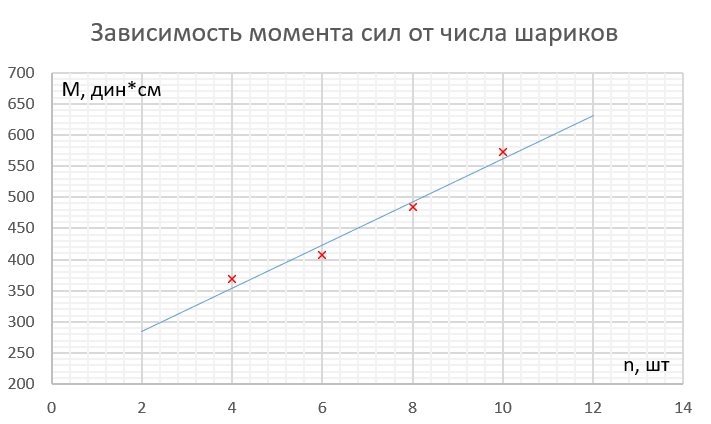
\includegraphics[width = 280pt]{image/graph2.png}
    \end{figure}

    Из МНК определяем угловой коэффициент $k$: $$k = 34,6 \pm 4,0 \;\text{дин}\cdot\text{см}.$$ Откуда рассчитаем величину вертикальной составляющей $B_v$ магнитного поля Земли: $$B_v = 0,81 \pm 0,01 \;\text{Гс}.$$

\subsection{Подсчёт индукции магнитного поля Земли}

Полная величина индукции $B$:
$$B = \sqrt{B_v^2+B_h^2} \approx 0,90 \pm 0,06\;\text{Гс}.$$

Магнитное наклонение $\beta$: 
$$\beta = arctan{\frac{B_v}{B_h}} \approx 63^\circ.$$

\section{Вывод}

\section{Контрольные вопросы}

 \end{document}